\documentclass{article}

\usepackage[margin=1in]{geometry}     %for 1inch margins that play nice with fancyhdr
\usepackage{amsmath,amssymb}          % math and junk
\usepackage{fancyhdr}                 % for a nice running header and footer
\usepackage{lastpage}                 % for nice "X of Y" footer
\usepackage[per-mode=symbol,alsoload=binary,detect-all=true]{siunitx}
                                      % for nice units and junk!
\usepackage{gnuplot-lua-tikz}         % enable tikz plots made from gnuplot
\usepackage{float}                    % [H] option for floats
\usepackage[american]{circuitikz}     % for teh circuit diagrams
\usepackage[hidelinks]{hyperref}                 % get those sweet, sweet, links
\usepackage{framed}                   % for framed titlepage
\usepackage{subfig}

\usetikzlibrary{shapes,arrows}

% unused, but common for other experiments
\usepackage{rotating}                 % for sideways stuff!
%\usepackage{cancel}                   % for `canceling out' parts of equations. fancy!
\usepackage{mdwlist}                  % itemize* and friends
%\usepackage{verbatim}                 % for \verbatiminput command and comment environment
%\usepackage[colorinlistoftodos]{todonotes}                % todo's, if used/needed
%\usepackage{multirow}                 % for multi-row spans in tabular environment


% values!
\newcommand{\docAuthor}{Sean Barag}
\newcommand{\docCoAuthor}{None}
\newcommand{\ta}{Yang Gao}
\newcommand{\docTitle}{Data Acquisition Exercise}
\newcommand{\courseName}{ECE-L304}
\newcommand{\labNum}{Step 4}
\newcommand{\labSec}{064}
\newcommand{\dueDate}{17 January 2012}
\newcommand{\perfDate}{8 February 2012}

% paths
\graphicspath{{$HOME/texmf/graphics/}}


% meta-data
\pdfinfo{
	/Title    (\labNum: \docTitle)
	/Author   (\docAuthor)
	/Keywords (\docTitle, \labNum)
}

% for fancy header
\pagestyle{fancy}
\lhead{\courseName\ $|$ \labSec}
\chead{\labNum: \docTitle}
\rhead{\docAuthor}
\cfoot{\thepage\ of \pageref{LastPage}}

% title info
\title{\courseName\ \labNum: \\ \docTitle}
\author{\docAuthor}
\date{}

% shortcuts, cause I'm lazy
\newcommand{\bs}[1]{\boldsymbol{#1}}
\newcommand{\tbf}[1]{\textbf{#1}}
\newcommand{\ttt}[1]{\texttt{#1}}

\begin{document}
% Cover page written by Bryndon Blackburn
% Originally written by Bryndon Blalckburn
\begin{titlepage}
	\begin{center}
		\includegraphics[scale = 0.50]{DrexelLogo.pdf}
	\end{center}

	\large
	\begin{framed}
		\begin{center}
			Electrical and Computer Engineering Dept. \\
			Electrical Engineering Laboratory IV, ECE-L304 \\
		\end{center}
	\end{framed} \vspace{50pt}

	\begin{description}
		\item[Title:]\labNum: \docTitle
		\item[Author:] \docAuthor
		\item[Partner:] \docCoAuthor
		\item[Instructor:] \ta
		\item[Section:] \labSec
		\item[Date Performed:] \perfDate
		\item[Date Due:] \dueDate
		\item[Date Received:]
	\end{description}
\end{titlepage}


% Blank page so two-sided printing leaves the cover page on its own sheet
\thispagestyle{empty}
\newpage
\mbox{}

\maketitle
\setcounter{page}{1} % fixes page numbering issues caused by cover sheet
\tableofcontents % this helps
%\newpage
%\listoffigures   % there's over 9000 figures

\newpage % I want the actual content to be at the top of a new page

\section{Introduction}
The entirety of ECE-L304 is devoted to the design, construction, and debugging
of a digital voice recorder.  By providing students with an opportunity to
complete a project of larger scale than anything they have previously
attempted, the course offers its students valuable skills and experience with a
long-term engineering project.

As the system uses digital storage in the form of a RAM chip, it is necessary
to convert all input audio from its native analog form to a digital
representation.  Similarly, the stored digital representation must be converted
back to an analog signal so that it can be correctly rendered by a speaker.
These conversions are performed by an analog to digital converter (ADC) and a
digital to analog converter (DAC), resepectively.
%
In order to ease the design process, students first complete a simple ADC and
DAC simulation.  This helps to remind students of the operating properties and
behaviors of the two converters, as well as providing a schematic similar to
the one required in the final design.

\section{Part 1}

Part one of step four required students to perform a rudimentary read-write
exercise using PSpice.  Using a~``RAM8kX8break'' RAM element paired with
several digital value generators, values were written to each of two different
memory addresses.

\subsection{Schematic}
As the lab instructions provided a functioning schematic for this system, it
has been reproduced here in Figure~\ref{f:schem1}.
%
\begin{figure}[H]
\centering
	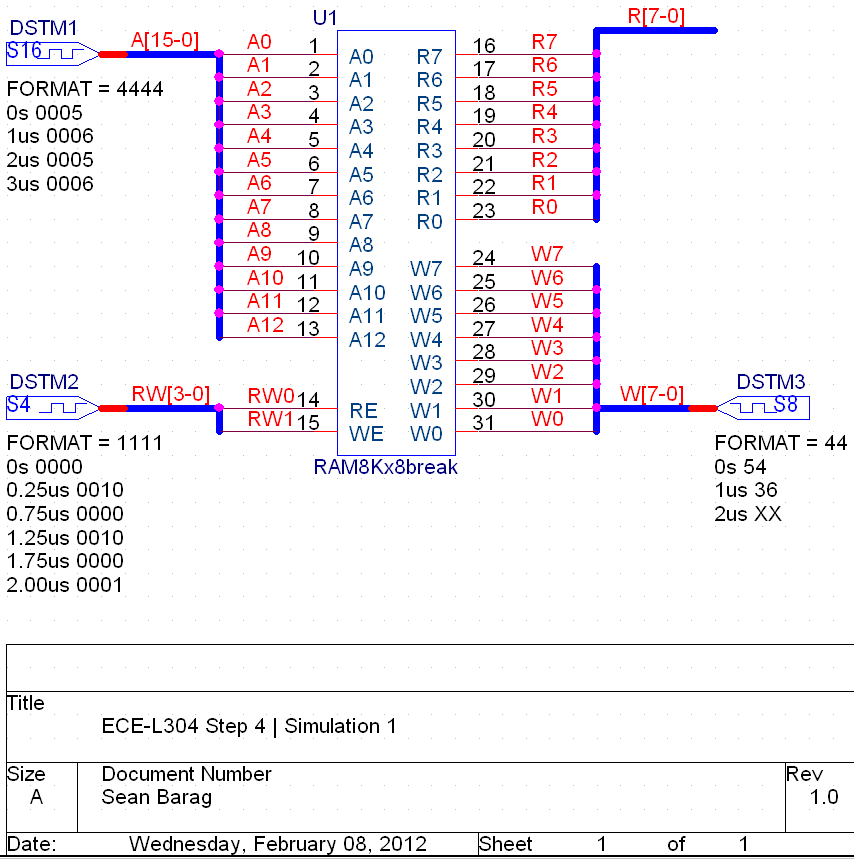
\includegraphics[width=.8\textwidth]{img/shot/schem1.png}
	\parbox{.8\textwidth}{
	\caption[Part 1 Schematic]{PSpice schematic for the circuit simulated in
	part one of step four.}
	\label{f:schem1}}
\end{figure}
%
The system writes the hex values \ttt{0x54} and \ttt{0x36} to the registers
located at \ttt{0x05} and \ttt{0x06}, respectively.  The values at these
locations are then read back to the \ttt{R} bus in the same sequence in which
they were written.

\subsection{Simulation}
For the sake of such a simple example, each read and write operation takes
just~\SI{1}{\micro\second}.  This allowed the student to simulate the circuit
over a convenient~\SI{4}{\micro\second} period while monitoring the values at
each data bus.  The plot produced by PSpice for this simulation is shown in
Figure~\ref{f:schem1plot}.
%
\begin{figure}[H]
\centering
	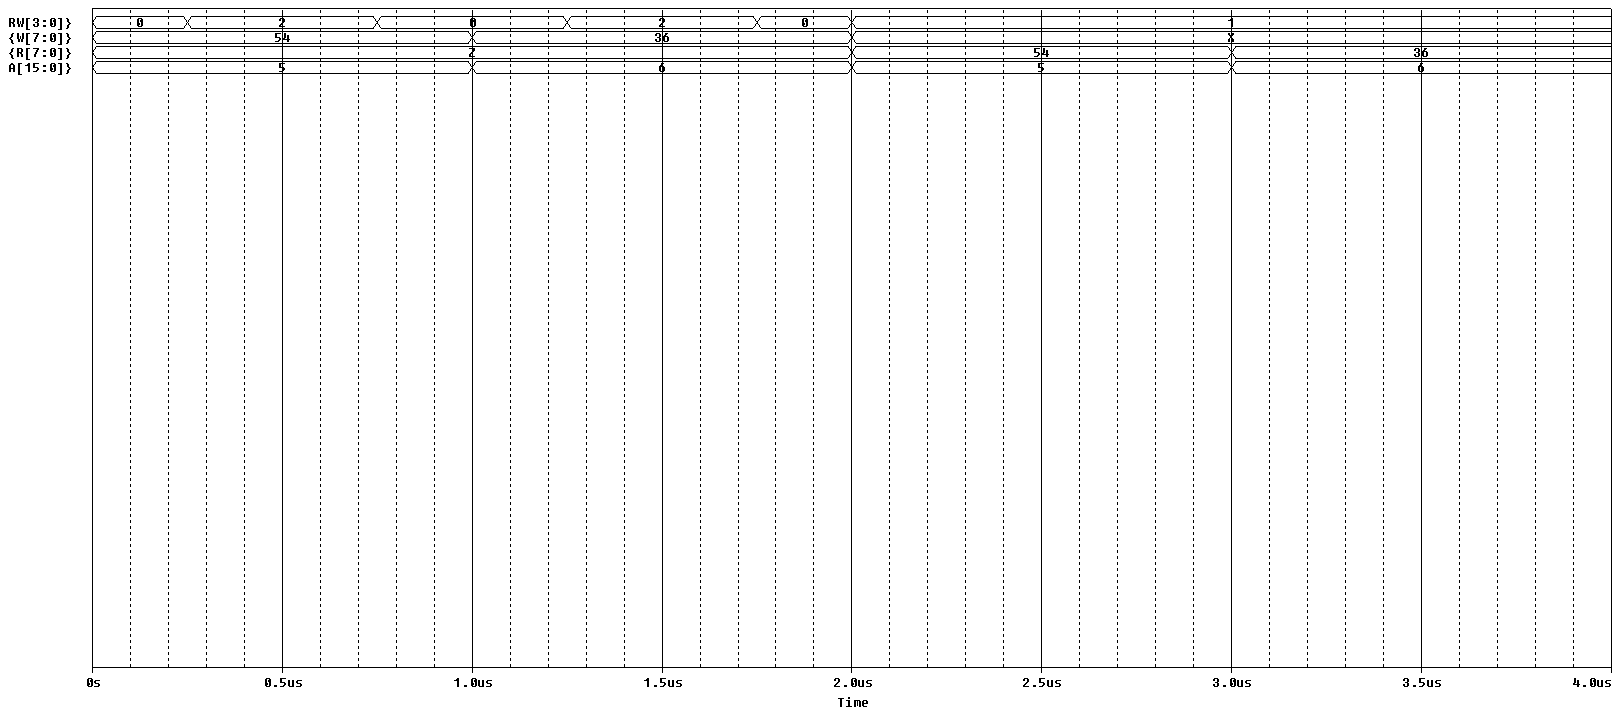
\includegraphics[width=.8\textwidth]{img/shot/sim1_plot.png}
	\parbox{.8\textwidth}{
	\caption[Part 1 Simulation Results]{Results of simulating the schematic
	shown in Figure~\ref{f:schem1} for~\SI{4}{\micro\second}.  A larger version
	of this figure is available in appendix Figure~\ref{f:schem1plot_big}.}
	\label{f:schem1plot}}
\end{figure}
%
The output of a hypothetical address generator is connected to the \ttt{A}
register, which changes value once per millisecond.  Note that the duplicate
addresses are present so that the system can read values from said addresses
after storing the value of \ttt{W} during the first occurrence of each address.
Reading and writing are enabled by the  \ttt{RW} register.  As the timing in
Figure~\ref{f:schem1} implies, writing is enabled for~\SI{0.5}{\micro\second}
across the center of each value from the \ttt{A} bus (i.e. from~$i +
\SI{0.25}{\micro\second}$ to~$i + \SI{0.75}{\micro\second}$.
After~\SI{2}{\milli\second}, \ttt{RW} enables reading for an infinite amount of
time.  As a result of these characteristics, it is safe to conclude that the
system follows all applicable read/write rules.

Figures~\ref{f:schem1plot} and~\ref{f:schem1plot_big} show that the system
correctly reads back the data it writes.  As such, the schematic can be
considered fully functional.

\section{Part 2}

The second part of step four builds on the skills obtained in part one,
requiring students to increase the number of memory addresses used and the size
of each stored value, while still creating an accurate reproduction of the data
after storage has been completed.

\subsection{Schematic}
Like with part one, the schematic for this expanded RAM use case was provided
in the lab instructions.  The schematic as simulated is included here in
Figure~\ref{f:schem2}.
%
\begin{figure}[H]
\centering
	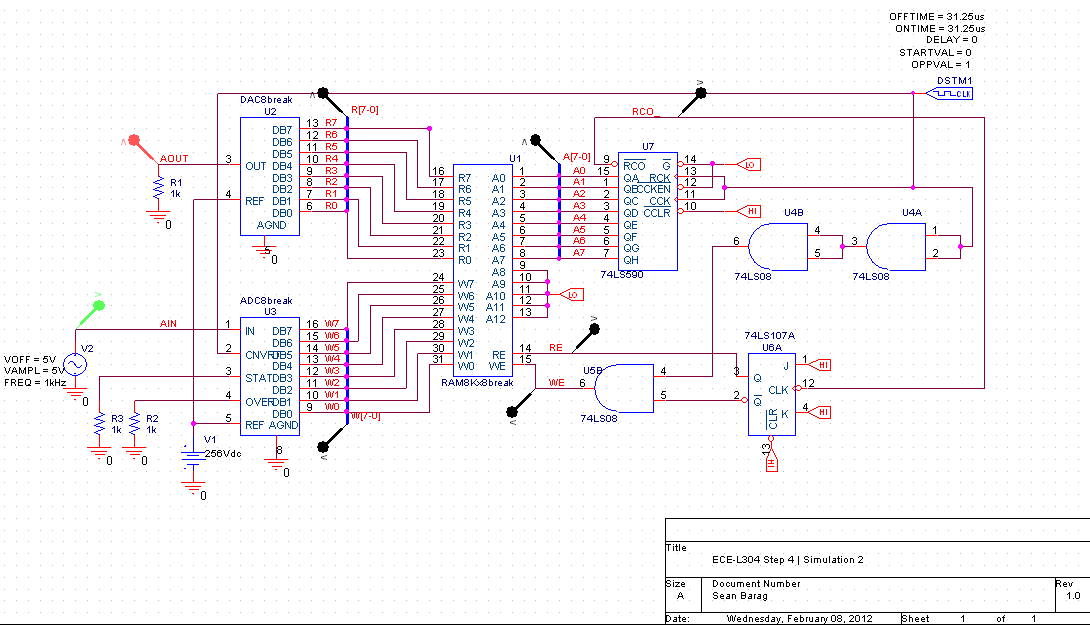
\includegraphics[width=.8\textwidth]{img/shot/schem2.png}
	\parbox{.8\textwidth}{
	\caption[Part 2 Schematic]{PSpice schematic for the circuit simulated in
	part two of step four.}
	\label{f:schem2}}
\end{figure}
%
The schematic shown reads~256 values of~8-bit data from the \ttt{W} register
(the output of an ADC) and stores them in addresses~\ttt{0x00}
through~\ttt{0xFF} in memory.  These values are subsequently read from those
locations and written to the \ttt{R} register for conversion to analog and
final output.

\subsection{Simulation}
This system has a clock period of~\SI{62.5}{\micro\second}, corresponding to a
clock frequency of~\SI{16}{\kilo\hertz}.  Since there are~256 addresses being
utilized~(each for both read and write), the simulation lasted
for
%
\begin{equation*}
\SI{256}{Addresses} \cdot \SI{2}{Accesses\per Address} \cdot
	\SI{62.5}{\micro\second\per Access} = \SI{32}{\milli\second} \quad \text{.}
\end{equation*}

Initially, the ADC and DAC were driven by a~\SI{256}{\volt} source.  The
resulting output, as calculated by PSpice, is shown in
Figure~\ref{f:schem2plot1}.
%
\begin{figure}[H]
\centering
	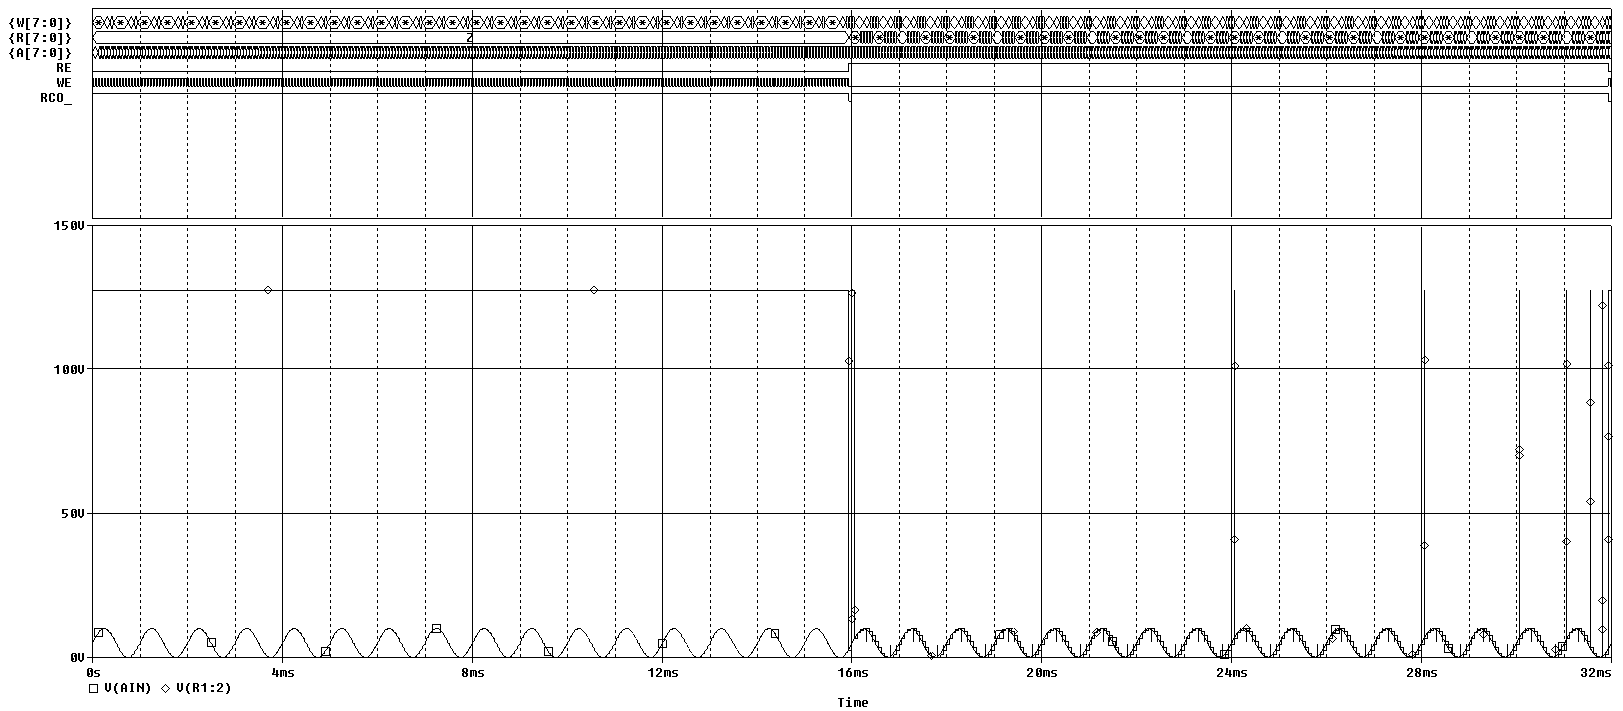
\includegraphics[width=.8\textwidth]{img/shot/sim2_plot1.png}
	\parbox{.8\textwidth}{
	\caption[Part 2 Simulation Results 1]{Results of simulating the schematic
	shown in Figure~\ref{f:schem2} for one full read-write cycle (in this
	case~\SI{32}{\milli\second}) with a~\SI{256}{\volt} supply.  A larger
	version of this figure is available in appendix
	Figure~\ref{f:schem2plot1_big}.}
	\label{f:schem2plot1}}
\end{figure}
%
While the output appears to represent the input fairly accurately, the output
is clamped at roughly~\SI{125}{\volt} while the system is reading data.
Additionally, there are occasional spikes in output voltage to the
same~\SI{125}{\volt} level that seem to correspond to addresses with only
consecutive ones in the most significant bits~(e.g. \ttt{1000 0000}, \ttt{1100
0000}, \ttt{1110, 000}, \ldots).  This phenomenon was prevented by changing the
ADC and DAC supplies to just~\SI{10}{\volt}, which produced the plot shown in
Figure~\ref{f:schem2plot2}.
%
\begin{figure}[H]
\centering
	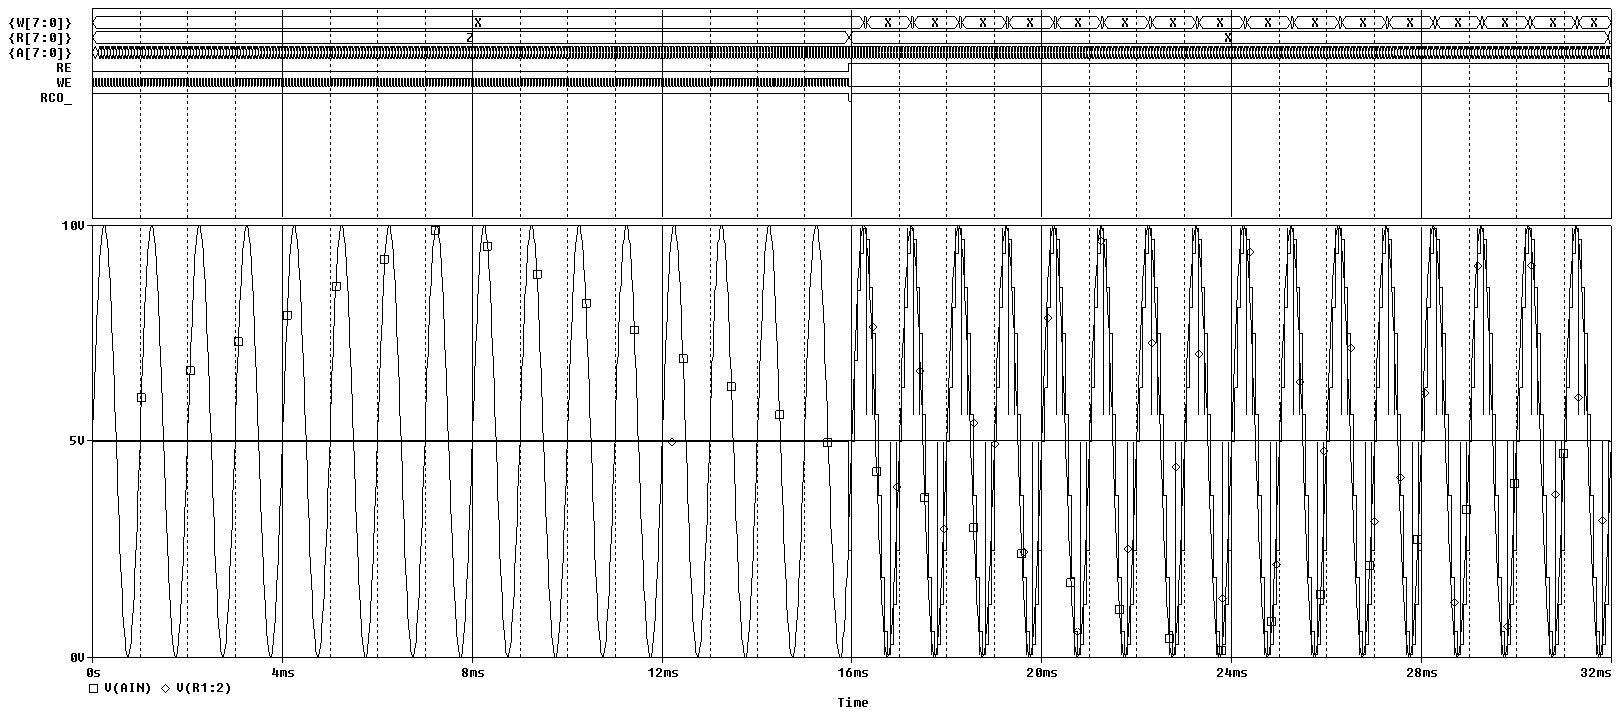
\includegraphics[width=.8\textwidth]{img/shot/sim2_plot2.png}
	\parbox{.8\textwidth}{
	\caption[Part 2 Simulation Results 2]{Results of simulating the schematic
	shown in Figure~\ref{f:schem2} for one full read-write cycle (in this
	case~\SI{32}{\milli\second}) for a supply voltage of~\SI{10}{\volt}.  A
	larger version of this figure is available in appendix
	Figure~\ref{f:schem2plot2_big}.}
	\label{f:schem2plot2}}
\end{figure}
%
After making this modification to the supply voltage, the output still clamps
to half the supply voltage while reading data.  Since this is
just~\SI{5}{\volt} now, there is no risk of damaging components.  While spikes
to half-supply voltage are still present, they are now periodic, and appear to
occur twice per period of sinusoidal input.  Regardless, the input and output
waveforms match well within the limitations of the~8 bit ADC and DAC
resolutions.  As this system is merely an extension of the one in part one, the
relationships between the \ttt{A}, \ttt{W}, \ttt{R}, and \ttt{RW} registers
remains the same, and the proper read/write timing rules are still followed.

After careful observation, it can be seen that there is a propagation delay for
values to pass through the L4S590 counter IC equal to the period of one full
clock cycle.  This is evident by the time between~$t = 0$ and the first
non-zero value plotted in Figures~\ref{f:schem2plot2}
and~\ref{f:schem2plot2_big}.  Similarly, there is a lag between when \ttt{RE}
goes high and when the first valid data is produced.  This is equal to two full
clock periods~(\SI{62.5}{\micro\second}); one for the counter to reset, and
another for the reset to propagate through the device.


%\section{Conclusions}

In conclusion, students simulated a fully functional RAM system in which data
was both stored to and retrieved from the~\SI{64}{kb} RAM chip.   Both the
rudimentary and complex systems exhibited the correct timing behavior, and
reproduced the input data accurately.  While the output of the 8-bit system in
part two showed some anomalies, they are acceptable for the purposes of a basic
voice recorder.  After tuning the complex design so that the anomalies were of
a safe voltage, both systems are ready to be implemented in hardware.



\newpage
\appendix
\section{Plots}

\begin{figure}[H]
\centering
	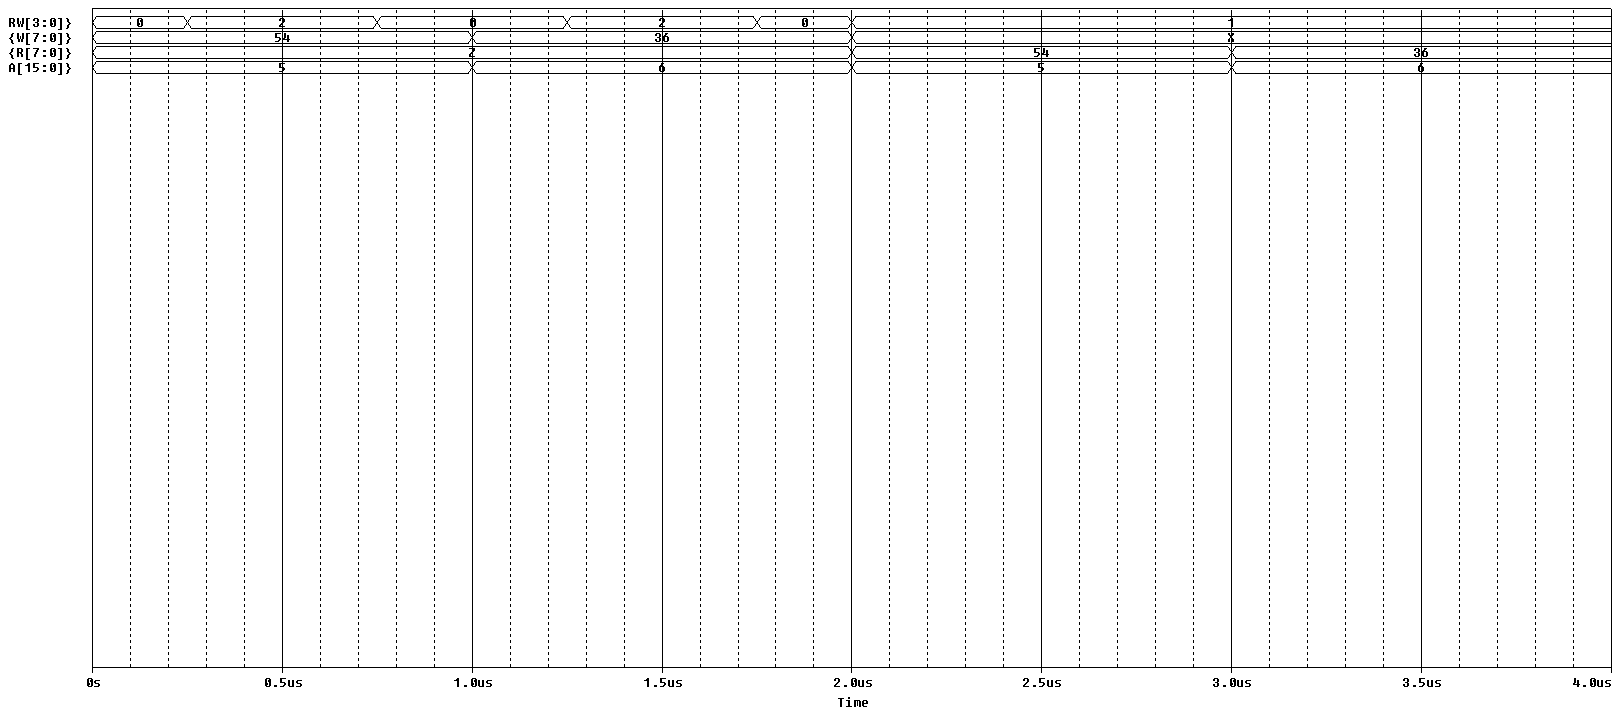
\includegraphics[angle=90, height=8in]{img/shot/sim1_plot.png}
	\parbox{.8\textwidth}{
	\caption[Part 1 Simulation Results (Full Size)]{Enlarged
	version of the plot shown in Figure~\ref{f:schem1plot}.}
	\label{f:schem1plot_big}}
\end{figure}

\begin{figure}[H]
\centering
	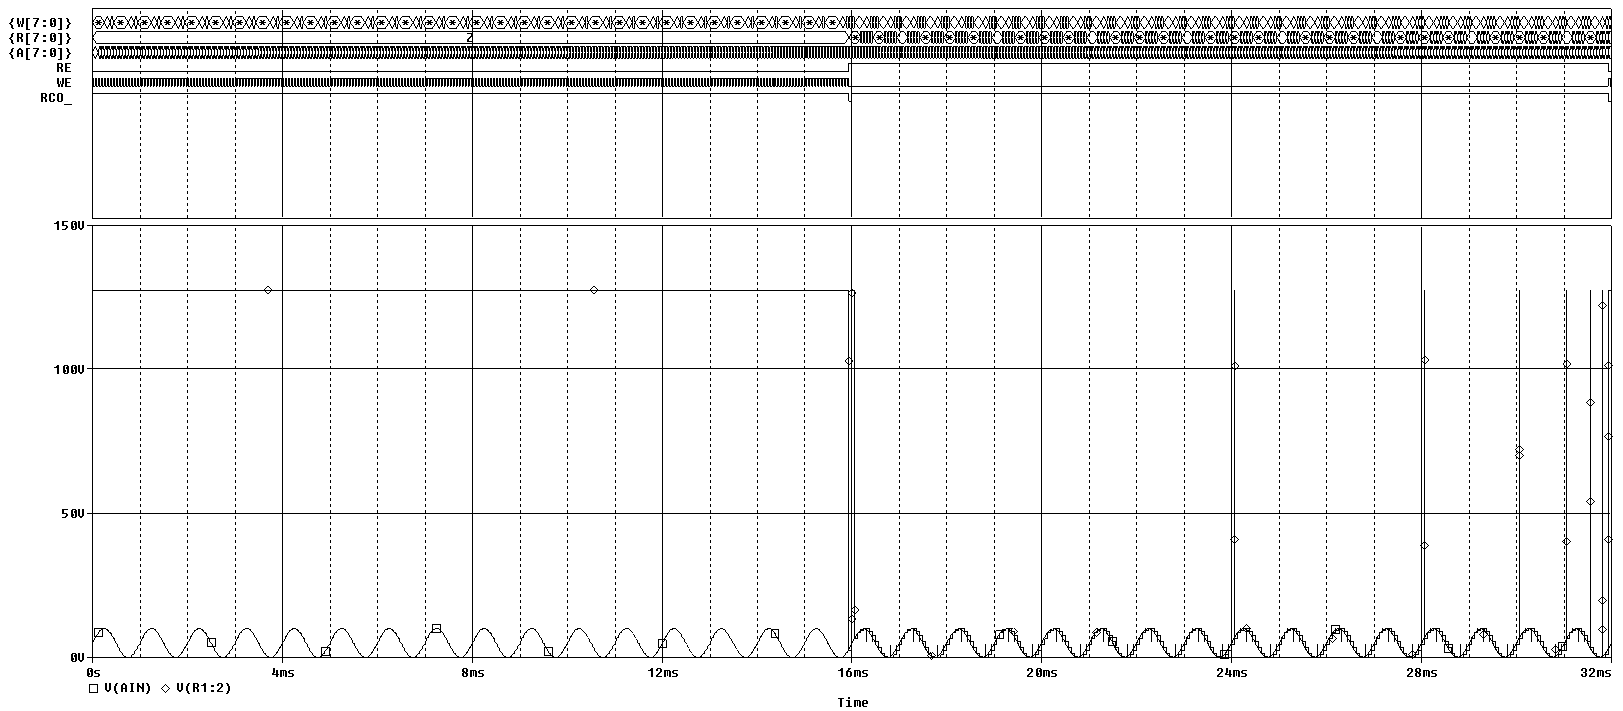
\includegraphics[angle=90, height=8in]{img/shot/sim2_plot1.png}
	\parbox{.8\textwidth}{
	\caption[Part 2 Simulation Results 1 (Full Size)]{Enlarged
	version of the plot shown in Figure~\ref{f:schem2plot1}.}
	\label{f:schem2plot1_big}}
\end{figure}

\begin{figure}[H]
\centering
	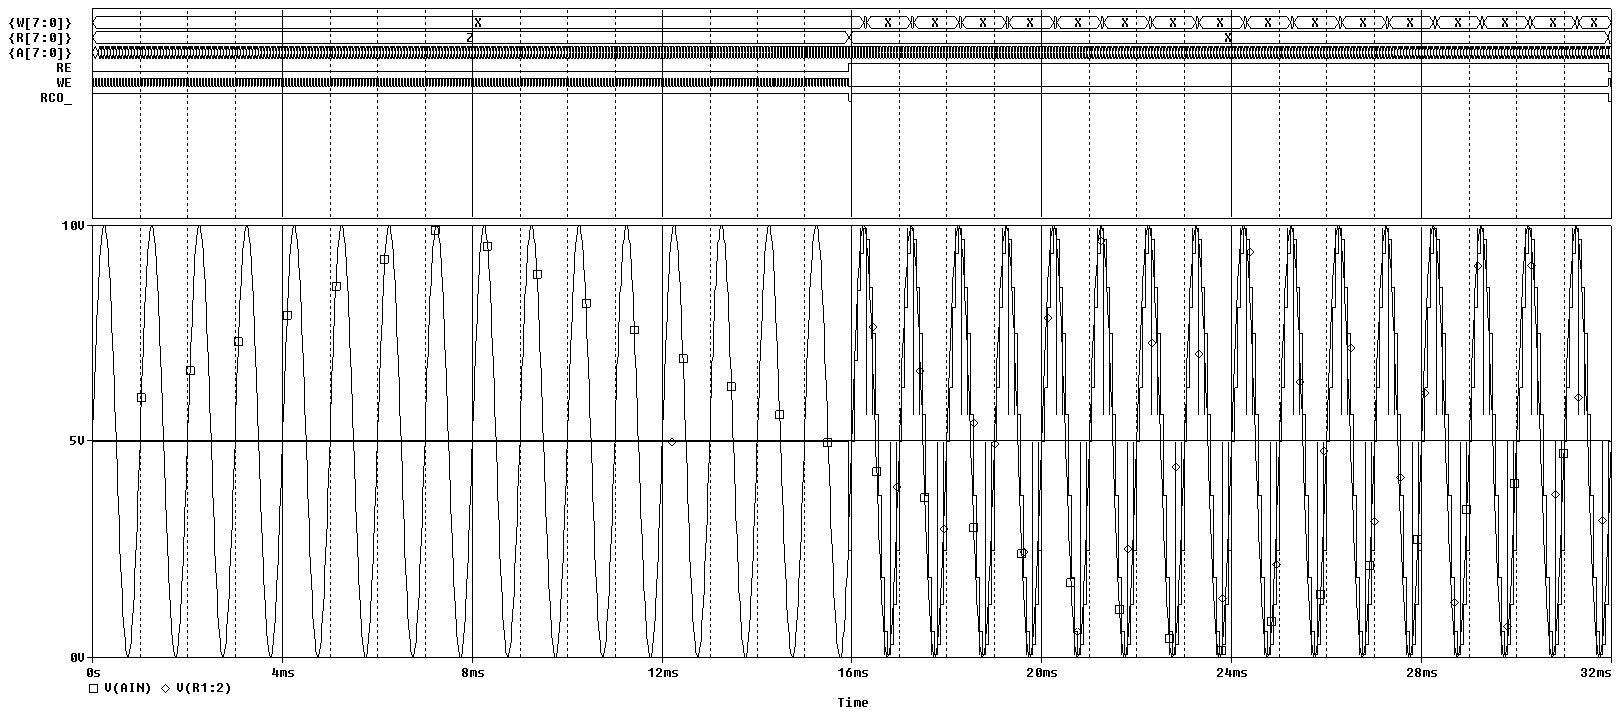
\includegraphics[angle=90, height=8in]{img/shot/sim2_plot2.png}
	\parbox{.8\textwidth}{
	\caption[Part 2 Simulation Results 2 (Full Size)]{Enlarged
	version of the plot shown in Figure~\ref{f:schem2plot2}.}
	\label{f:schem2plot2_big}}
\end{figure}

\section{License}

Copyright \copyright\ 2011, Sean Barag.  All rights reserved.

Redistribution and use in source and binary forms, with or without
modification, are permitted provided that the following conditions are met:
\begin{itemize}
\item Redistributions of source code must retain the above copyright notice, this
  list of conditions and the following disclaimer.
\item Redistributions in binary form must reproduce the above copyright notice, this
  list of conditions and the following disclaimer in the documentation and/or
  other materials provided with the distribution.
\item Neither the name of the owner nor the names of its contributors may be
  used to endorse or promote products derived from this software without specific
  prior written permission.
\end{itemize}

THIS SOFTWARE IS PROVIDED BY THE COPYRIGHT HOLDERS AND CONTRIBUTORS ``AS IS'' AND
ANY EXPRESS OR IMPLIED WARRANTIES, INCLUDING, BUT NOT LIMITED TO, THE IMPLIED
WARRANTIES OF MERCHANTABILITY AND FITNESS FOR A PARTICULAR PURPOSE ARE
DISCLAIMED. IN NO EVENT SHALL THE COPYRIGHT HOLDER OR CONTRIBUTORS BE LIABLE
FOR ANY DIRECT, INDIRECT, INCIDENTAL, SPECIAL, EXEMPLARY, OR CONSEQUENTIAL
DAMAGES (INCLUDING, BUT NOT LIMITED TO, PROCUREMENT OF SUBSTITUTE GOODS OR
SERVICES; LOSS OF USE, DATA, OR PROFITS; OR BUSINESS INTERRUPTION) HOWEVER
CAUSED AND ON ANY THEORY OF LIABILITY, WHETHER IN CONTRACT, STRICT LIABILITY,
OR TORT (INCLUDING NEGLIGENCE OR OTHERWISE) ARISING IN ANY WAY OUT OF THE USE
OF THIS SOFTWARE, EVEN IF ADVISED OF THE POSSIBILITY OF SUCH DAMAGE.\\

Source code for this document is available at \texttt{http://github.com/sjbarag/}.



\end{document}
